\section{Ábacos}

\begin{frame}[fragile]{Contexto histórico}

    \begin{itemize}
        \item As máquinas de Turing tem muitas limitações: uma delas é trabalhar exclusivamente
            com inteiros positivos, o que exclui o zero

        \item Além disso, elas foram propostas antes do surgimento dos computadores digitais

        \item De fato, as máquinas de Turing contribuíram significativamente no desenvolvimento
            destes computadores

        \item Uma importante característica presente nos computadores digitais e ausentes nas
            máquinas de Turing é o acesso aleatório à memória

        \item Além disso, o sistema numérico subjacente é o sistema binário, e não o monádico

        \item O acréscimo destas duas características às máquinas de Turing levam aos ábacos
    \end{itemize}

\end{frame}

\begin{frame}[fragile]{Ábaco}

    \begin{block}{Definição}
        Uma \textbf{máquina de Lambek} ou uma \textbf{máquina de ábaco} é uma versão idealizada
        de computador, com as seguintes características:
        \begin{enumerate}[(a)]
            \item acesso ao um número \textbf{ilimitado} de registradores $R_0, R_1, R_2, \ldots$
            \item cada registrador pode armazenar um número natural (positivos e o zero) de tamanho
                \textbf{arbitrário}
            \item cada registrador tem seu próprio \textbf{endereço}, de modo que é possível se 
                mover do registrador $R_i$ para o registrador $R_j$ diretamente, sem precisar 
                passar, passo a passo, pelos registradores intermediários 
                $R_{i + 1}, R_{i + 2}, \ldots, R_{j - 1}$
        \end{enumerate}
    \end{block}

\end{frame}

\begin{frame}[fragile]{Notação}

    \begin{itemize}
        \item Os registradores são representados pela letra maiúscula $R$ e pelo subscrito $i$,
            indicando o número do registrador

        \item A notação $[m]$ indica o número que está armazenado no registrador $R_m$

        \item Um registrador pode estar vazio, isto é, armazenar o valor zero

        \item A instrução ``{\it Coloque a soma dos números armazenados em $R_m$ e em $R_n$ em 
            $R_p$} pode ser escrita como
        \[
            [m] + [n] \to p
        \]

        \item O número à direita da seta indica o registrador que armazenará o resultado da
            instrução
    \end{itemize}

\end{frame}

\begin{frame}[fragile]{Programas em ábaco}

    Um \textbf{programa} em um ábaco consiste em uma lista de instruções numeradas. Cada
    uma destas instruções é de uma das duas formas abaixo:

    \begin{small}
    \vspace{0.2in}

    \[
        (q)\ \ \mbox{acrescente um à caixa $m$ e vá para a instrução $r$}
    \]
    \end{small}

    \vspace{0.1in}
    ou
    \vspace{0.1in}

    \begin{small}
    \[
        (q)\ \ \left\lbrace \begin{array}{ll}
            \mbox{se a caixa $m$ não está vazia},& \mbox{então subtraia um da caixa $m$ e vá para $r$}\\
            \mbox{se a caixa $m$ está vazia},& \mbox{então vá para $s$}\\
        \end{array}\right.
    \]
    \end{small}

\end{frame}

\begin{frame}[fragile]{Diagramas correspondentes às duas instruções dos ábacos}

    \renewcommand{\figurename}{Instrução}
    \begin{minipage}{0.45\textwidth}
    \begin{figure}[h]
        \centering
        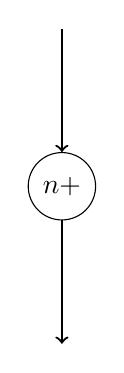
\begin{tikzpicture}
            \coordinate (A) at (0, 4);
            \node[draw,circle] (B) at (0, 2) { $n+$ };
            \coordinate (C) at (0, 0);

            \draw[thick,->] (A) -- (B);
            \draw[thick,->] (B) -- (C);
        \end{tikzpicture}
        \caption{Acrescente um ao número armazenado no registrador $R_n$}
    \end{figure}
    \end{minipage}
    \begin{minipage}{0.45\textwidth}
    \begin{figure}[h]
        \centering
        \begin{tikzpicture}
            \coordinate (A) at (0, 4);
            \node[draw,circle] (B) at (0, 2) { $n-$ };
            \coordinate (C) at (-2, 0);
            \coordinate (D) at (2, 0);

            \draw[thick,->] (A) -- (B);
            \draw[thick,->] (B) -- (C);
            \draw[thick,->] (B) -- node[anchor=west] { $e$ } (D);
        \end{tikzpicture}
        \caption{Se $R_n$ estiver vazio, saia pela seta $e$; caso contrário, subtraia
            um e saia pela outra seta}
    \end{figure}
    \end{minipage}


\end{frame}
